% Source for the figure of MPSCQueue (sec. 24.3): two lanes of blocks of 4
% places, each block with the count f of the items written, the places of
% the consumer (below) and of the producer (above), and a block that the
% consumer gave back to the first lane, on its stack of blocks to reuse.
% Build: make figures (in ../build).
\documentclass[border=4pt]{standalone}
\usepackage[T1]{fontenc}
\usepackage{newpxtext,newpxmath}
\usepackage[varqu,varl,scaled=0.95]{zi4}
\usepackage{tikz}
% tikz-ads.tex: the TikZ styles shared by the figures of the memory of the
% manual, \input by each standalone figure: a cell of a vector (cell), the
% cell that an operation touches (touched), a free cell (free), a node of a
% linked structure (node), the labels of indices (index) and of variables
% (var), a pointer (ptr), and \cells and \indices to draw a row of cells.
\usetikzlibrary{arrows.meta,positioning,calc,fit,shapes.multipart}
\definecolor{adsTouched}{RGB}{214,196,236}
\definecolor{adsFree}{RGB}{236,236,236}
\tikzset{
  ads/.style={>={Stealth[length=2mm]},font=\small,
              every node/.append style={inner sep=0pt}},
  cell/.style={draw,minimum width=7mm,minimum height=7mm,
               font=\small\ttfamily,outer sep=0pt},
  touched/.style={cell,fill=adsTouched},
  free/.style={cell,fill=adsFree,text=black!45},
  node/.style={draw,rounded corners=1pt,minimum width=8mm,
               minimum height=6mm,font=\small\ttfamily},
  index/.style={font=\scriptsize\ttfamily,text=black!60},
  var/.style={font=\small\itshape},
  ptr/.style={->,thick}
}
% \cells{name}{x,y}{list}: a row of cells, the first at (x,y), named
% name-0, name-1, ...; each item is text/style, the style one of cell,
% touched and free (e.g., {a/cell,e/touched,/free})
\newcommand{\cells}[3]{%
  \foreach \v/\s [count=\i from 0] in {#3}
    \node[\s] (#1-\i) at ($(#2)+(\i*7mm,0)$) {\v};}
% \indices{name}{n}: the indices 0 .. n-1 under the cells of name
\newcommand{\indices}[2]{%
  \foreach \i in {0,...,\numexpr#2-1\relax}
    \node[index,below=1.2mm of #1-\i] {\i};}

\begin{document}
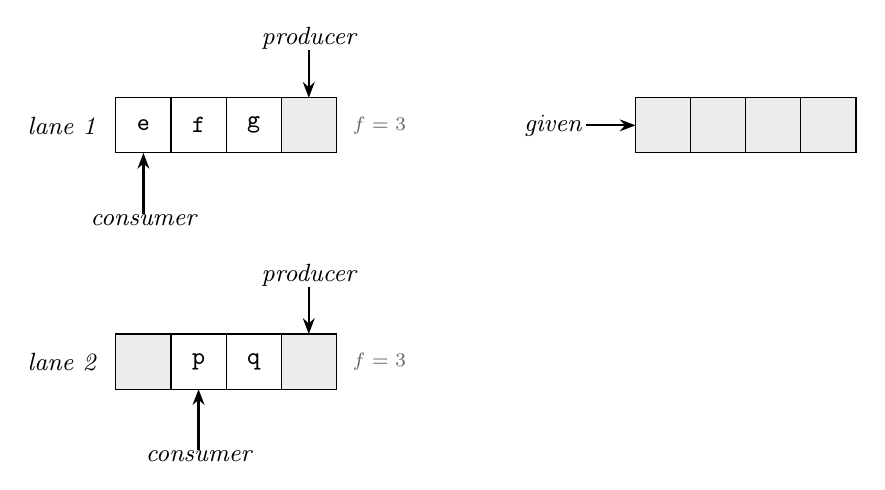
\begin{tikzpicture}[ads]
  \node[var,anchor=east] at (-6mm,0) {lane 1};
  \cells{B}{0,0}{e/cell,f/cell,g/cell,/free}
  \node[index,anchor=west] at ($(B-3.east)+(2mm,0)$) {$f = 3$};
  \node[var] (out1) at ($(B-0)+(0,-12mm)$) {consumer};
  \draw[ptr] (out1) -- (B-0.south);
  \node[var] (in1) at ($(B-3)+(0,11mm)$) {producer};
  \draw[ptr] (in1) -- (B-3.north);
  \node[var,inner sep=1.5pt] (gv) at (52mm,0) {given};
  \cells{A}{66mm,0}{/free,/free,/free,/free}
  \draw[ptr] (gv) -- (A-0.west);
  \node[var,anchor=east] at (-6mm,-30mm) {lane 2};
  \cells{C}{0,-30mm}{/free,p/cell,q/cell,/free}
  \node[index,anchor=west] at ($(C-3.east)+(2mm,0)$) {$f = 3$};
  \node[var] (out2) at ($(C-1)+(0,-12mm)$) {consumer};
  \draw[ptr] (out2) -- (C-1.south);
  \node[var] (in2) at ($(C-3)+(0,11mm)$) {producer};
  \draw[ptr] (in2) -- (C-3.north);
\end{tikzpicture}
\end{document}
